\documentclass[12pt]{beamer}
\usepackage{../Estilos/BeamerMAF}
\usepackage{../Estilos/ColoresLatex}

\usetheme{Dresden}
\usecolortheme{seahorse}
%\useoutertheme{default}
\setbeamercovered{invisible}
% or whatever (possibly just delete it)
\setbeamertemplate{section in toc}[sections numbered]
\setbeamertemplate{subsection in toc}[subsections numbered]
\setbeamertemplate{subsection in toc}{\leavevmode\leftskip=3.2em\rlap{\hskip-2em\inserttocsectionnumber.\inserttocsubsectionnumber}\inserttocsubsection\par}
\setbeamercolor{section in toc}{fg=blue}
\setbeamercolor{subsection in toc}{fg=blue}
\setbeamercolor{frametitle}{fg=blue}
\setbeamertemplate{caption}[numbered]

\setbeamertemplate{footline}
\beamertemplatenavigationsymbolsempty
\setbeamertemplate{headline}{}

\makeatletter
\setbeamercolor{section in foot}{bg=gray!30, fg=black!90!orange}
\setbeamercolor{subsection in foot}{bg=blue!30!yellow, fg=red}
\setbeamertemplate{footline}
{
  \leavevmode%
  \hbox{%
  \begin{beamercolorbox}[wd=.333333\paperwidth,ht=2.25ex,dp=1ex,center]{section in foot}%
    \usebeamerfont{section in foot} \insertsection
  \end{beamercolorbox}}%
  \begin{beamercolorbox}[wd=.333333\paperwidth,ht=2.25ex,dp=1ex,center]{subsection in foot}%
    \usebeamerfont{subsection in foot}  \insertsubsection
  \end{beamercolorbox}%
  \begin{beamercolorbox}[wd=.333333\paperwidth,ht=2.25ex,dp=1ex,right]{date in head/foot}%
    \usebeamerfont{date in head/foot} \insertshortdate{} \hspace*{2em}
    \insertframenumber{} / \inserttotalframenumber \hspace*{2ex} 
  \end{beamercolorbox}}%
  \vskip0pt%
\makeatother 

\makeatletter
\patchcmd{\beamer@sectionintoc}{\vskip1.5em}{\vskip0.8em}{}{}
\makeatother


\setbeamercolor{section in foot}{bg=ao(english), fg=white}
\setbeamercolor{subsection in foot}{bg=ao, fg=white}
\setbeamercolor{date in foot}{bg=goldenrod, fg=white}

\makeatletter
\setbeamertemplate{footline}
{
\leavevmode%
\hbox{%
\begin{beamercolorbox}[wd=.333333\paperwidth,ht=2.25ex,dp=1ex,center]{section in foot}%
  \usebeamerfont{section in foot} \insertsection
\end{beamercolorbox}%
\begin{beamercolorbox}[wd=.333333\paperwidth,ht=2.25ex,dp=1ex,center]{subsection in foot}%
  \usebeamerfont{subsection in foot}  \insertsubsection
\end{beamercolorbox}%
\begin{beamercolorbox}[wd=.333333\paperwidth,ht=2.25ex,dp=1ex,right]{date in head/foot}%
  \usebeamerfont{date in head/foot} \insertshortdate{} \hspace*{1.5em}
  \insertframenumber{} / \inserttotalframenumber \hspace*{2ex} 
\end{beamercolorbox}}%
\vskip0pt%
}
\makeatother
% \usefonttheme{serif}
\resetcounteronoverlays{saveenumi}

\AtBeginDocument{\RenewCommandCopy\qty\SI}
\ExplSyntaxOn
\msg_redirect_name:nnn { siunitx } { physics-pkg } { none }
\ExplSyntaxOff


\date{16 de octubre de 2025}
\title{\large{Ortogonalización Gram-Schmidt}}
\subtitle{Polinomios de Chebyshev Tipo II}
\author{M. en C. Gustavo Contreras Mayén}

\begin{document}
\maketitle
\fontsize{14}{14}\selectfont
\spanishdecimal{.}

\section*{Contenido}
\frame{\frametitle{Contenido} \tableofcontents[currentsection, hideallsubsections]}

\section{Ejercicio}
\frame{\frametitle{Temas a revisar} \tableofcontents[currentsection, hideothersubsections]}
\subsection{Enunciado}

\begin{frame}
\frametitle{Enunciado del problema}
Con el método de ortogonalización de Gram-Schmidt construye los primeros tres polinomios de Chebyshev de Tipo II.
\end{frame}
\begin{frame}
\frametitle{Elementos para el procedimiento}
Considera lo siguiente:
\pause
\begin{table}
\begin{tabular}{l l}
Funciones l. i. & $u_{n}(x) = x^{n}$ \\
 & $n = 0, 1, 2, \ldots$ \\ \pause
Intervalo & $-1 \leq x \leq 1$ \\ \pause
Función de peso & $\omega (x) = (1 -x^{2})^{\frac{1}{2}}$
\end{tabular}
\end{table}
\end{frame}

\subsection{Normalización}

\begin{frame}
\frametitle{Normalización de los polinomios de Chebyshev}
La normalización de los polinomios de Chebyshev de tipo II $U_{n}(x)$, está dada por la expresión:
\pause
\begin{align*}
\scaleint{6ex}_{\bs -1}^{1} \, U_{m}(x) \, U_{n} (x) \, \omega (x) \dd{x} = \delta_{mn} \, \dfrac{\pi}{2}
\end{align*}
\end{frame}
\begin{frame}
\frametitle{Normalización a considerar}
Dada la normalización de los $U_{n}$, hay que tomar en cuenta que:
\pause
\begin{eqnarray*}
&\scaleint{5ex}_{\bs a}^{b} \left[ \varphi_{j} (x) \right]^{2} \, \omega (x) \dd{x} = \\[0.5em] \pause
&\scaleint{6ex}_{\bs -1}^{1} \, U_{m}(x) \, U_{n} (x) \, \omega (x) \dd{x} = \\[0.5em] \pause
&= \delta_{mn} \, \dfrac{\pi}{2} = \pause N_{j}^{2}
\end{eqnarray*}
\end{frame}
\begin{frame}
\frametitle{Expresión para normalizar}
Entonces tenemos que:
\pause
\begin{align*}
\varphi_{i} (x) =  N_{i} \: \dfrac{\psi_{i} (x)}{ \bigg[ \displaystyle \scaleint{5ex} \psi_{i}^{2} \, \omega \dd{x} \bigg]^{1/2}}
\end{align*}
\end{frame}
\begin{frame}
\frametitle{Los términos $a_{i,j}$}
Los términos $a_{i,j}$ resultan:
\pause
\begin{align}
a_{i, j} = - \dfrac{ \displaystyle \scaleint{5ex} u_{i} \, \varphi_{j} \, \omega \dd{x}}{N_{j}^{2}}
\label{eq:ecuacion_10_49a}
\end{align}
\end{frame}    

\subsection*{Integral de apoyo}

\begin{frame}
\frametitle{Integral de apoyo}
Para reducir el tiempo en el cálculo de algunas integrales, nos apoyaremos con el siguiente resultado:
\pause
\begin{align*}
\scaleint{6ex}_{\bs -1}^{1} &x^{2n} \, (1 {-} x^{2})^{\frac{1}{2}} {=} \\[0.5em]
&= \begin{cases}
\dfrac{\pi}{2} \, \dfrac{1 \cdot 3 \cdot 5 \cdots (2 \, n {-} 1)}{4 \cdot 6 \cdot 8 \cdots (2 \, n {+} 2)} & n {=} 1, 2, \ldots \\[1em]
\dfrac{\pi}{2} & n {=} 0
\end{cases}
\end{align*}
\end{frame}

\section{Cambiando el valor de \texorpdfstring{$n$}{n}}
\frame{\frametitle{Temas a revisar} \tableofcontents[currentsection, hideothersubsections]}
\subsection{Caso \texorpdfstring{$n=0$}{n=0}}

\begin{frame}
\frametitle{Comenzando con el procedimiento}
Al seguir la técnica de ortogonalización, \pause hacemos que $n = 0$:
\pause
\begin{eqnarray*}
\begin{aligned}
\Rightarrow u_{0} (x) &=  x^{0} = \pause 1 \\[0.5cm] \pause
\Rightarrow \psi_{0} (x) &= u_{0} (x) = \pause  1 \\[0.5em] \pause
\Rightarrow \varphi_{0} (x) &= \dfrac{N_{0} \, \psi_{0} (x)}{\bigg[ \scaleint{6ex}_{-1}^{1} \big[ \psi_{0} (x) \big]^{2} \omega (x) \dd{x} \bigg]^{\frac{1}{2}}} = 
\end{aligned}
\end{eqnarray*}
\end{frame}
\begin{frame}
\frametitle{Resolviendo las operaciones}
\begin{align*}
\Rightarrow \varphi_{0} (x) = \dfrac{N_{0}}{\bigg[ \scaleint{6ex}_{-1}^{1} (1 -x^{2})^{\frac{1}{2}} \dd{x} \bigg]^{\frac{1}{2}}} =
\end{align*}
El valor de $N_{0}$ es:
\pause
\begin{align*}
N_{0}^{2} &= \dfrac{\pi}{2}
\end{align*}
\end{frame}
\begin{frame}
\frametitle{Resolviendo las operaciones}
La integral del denominador resulta (usamos a integral de apoyo):
\pause
\begin{eqnarray*}
\begin{aligned}
\bigg[ \scaleint{6ex}_{\bs -1}^{1} (&1 - x^{2})^{\frac{1}{2}} \bigg]^{\frac{1}{2}} = \pause \bigg[ \dfrac{\pi}{2} \bigg]^{\frac{1}{2}} \\[0.5em] \pause
&\Rightarrow \varphi_{0}(x) = \pause \dfrac{\sqrt{\pi/2}}{\sqrt{\pi/2}} = \pause 1
\end{aligned}
\end{eqnarray*}
\end{frame}
\begin{frame}
\frametitle{Primer resultado}
Se tiene entonces que la primera función ortogonal correspondiente a los polinomios de Chebyshev de tipo II es:
\pause
\begin{align*}
\setlength{\fboxsep}{3\fboxsep}\boxed{
\varphi_{0} (x) = 1}
\end{align*}
\end{frame}

\subsection{Caso \texorpdfstring{$n=1$}{n=1}}

\begin{frame}
\frametitle{Siguiente valor de $n$}
Continuamos la técnica ahora con el valor de $n = 1$
\pause
\begin{eqnarray*}
\begin{aligned}
\Rightarrow u_{1} (x) &= x^{1} = x \\[0.5cm] \pause
\Rightarrow \psi_{1} (x) &=  u_{1} + a_{1,0} \, \varphi_{0} \\[0.5em] \pause
a_{1,0} &= - \dfrac{\scaleint{5ex} u_{1} \, \varphi_{0} \, \omega \dd{x}}{(N_{0})^{2}} = \pause
- \dfrac{\scaleint{5ex}_{\bs -1}^{1} x \, (1 - x^{2})^{\frac{1}{2}} \dd{x}}{\dfrac{\pi}{2}} = \\[0.5em] \pause
&= 0 \hspace{1.5cm} \text{¿por qué la integral se anula?}
\end{aligned}
\end{eqnarray*}    
\end{frame}
\begin{frame}
\frametitle{Siguiente valor de $n$}
\begin{eqnarray*}
\begin{aligned}
\Rightarrow \quad &\psi_{1} (x) =  x \\[0.5em] \pause
\Rightarrow \quad &\varphi_{1} (x) = \dfrac{N_{1} \, \psi_{1} (x)}{\bigg[ \scaleint{6ex}_{\bs -1}^{1} [\psi_{1} (x)]^{2} \, \omega (x) \dd{x} \bigg]^{\frac{1}{2}}} \\[0.5em] \pause
&(N_{1})^{2} = \dfrac{\pi}{2}
\end{aligned}
\end{eqnarray*}    
\end{frame}
\begin{frame}
\frametitle{Siguiente valor de $n$}
Calculamos el valor de la integral en el denominador (usamos nuevamente la integral de apoyo):
\pause
\begin{eqnarray*}
\begin{aligned}
&\scaleint{6ex}_{\bs -1}^{1} x^{2} \, (1 - x^{2})^{\frac{1}{2}} \dd{x} = \pause \dfrac{\pi}{8} \\[0.4em] \pause
\Rightarrow \quad &\varphi_{1} (x) = \dfrac{x \, \sqrt{\pi/2}}{\sqrt{\pi/8}} = \pause 2 \, x
\end{aligned}
\end{eqnarray*}    
\end{frame}
\begin{frame}
\frametitle{Segundo resultado}
Hemos calculado la segunda función ortogonal correspondiente a los polinomios de Chebyshev de tipo II:
\pause
\begin{align*}
\setlength{\fboxsep}{3\fboxsep}\boxed{
\varphi_{2} (x) = 2 \, x}
\end{align*}
\end{frame}

\subsection{Caso \texorpdfstring{$n = 2$}{n = 2}}

\begin{frame}
\frametitle{Siguiente valor de $n$}
Continuamos la técnica ahora con el valor de $n = 2$:
\pause
\begin{eqnarray*}
\begin{aligned}
\Rightarrow u_{2} (x) &= x^{2} \\[0.5em] \pause
\Rightarrow \psi_{2} (x) &=  u_{2} + a_{2,0} \, \varphi_{0} + a_{2,1} \, \varphi_{1}
\end{aligned}
\end{eqnarray*}    
\end{frame}
\begin{frame}
\frametitle{Valor de los coeficientes}
Donde los coeficientes son:
\pause
\begin{eqnarray*}
\begin{aligned}    
a_{2,0} &= \pause - \dfrac{\scaleint{5ex} u_{2} \, \varphi_{0} \, \omega \dd{x}}{\big( N_{0} \big)^{2}} = \pause - \dfrac{\scaleint{5ex} x^{2} (1 - x^{2})^{\frac{1}{2}} \dd{x}}{\dfrac{\pi}{2}} = \pause - \dfrac{1}{4} \\[0.5em] \pause
a_{2,1} &= \pause - \dfrac{\scaleint{5ex} u_{2} \, \varphi_{1} \, \omega \dd{x}}{\big( N_{1} \big)^{2}} = \pause
- \dfrac{2 \scaleint{5ex} x^{3} (1 - x^{2})^{\frac{1}{2}} \dd{x}}{\dfrac{\pi}{2}} = \pause 0
\end{aligned}
\end{eqnarray*}
Revisa que usamos la integral de apoyo.
\end{frame}
\begin{frame}
\frametitle{Avanzando con la técnica}
Por lo que:
\pause
\begin{align*}
\psi_{2}(x) = x^{2} - \dfrac{1}{4}
\end{align*}
\pause
Entonces ya podemos calcular:
\pause
\begin{align*}
\varphi_{2}(x) = \dfrac{N_{2} \, \psi_{2} (x)}{ \bigg[ \scaleint{5ex} [\psi_{2} (x)]^{2} \omega (x) \dd{x} \bigg]^{\frac{1}{2}}}
\end{align*}
\end{frame}
\begin{frame}
\frametitle{Obteniendo $\varphi_{2}(x)$}
Presentamos la expresión para obtener la tercera función ortogonal:
\pause
\begin{eqnarray*}
\begin{aligned}
\varphi_{2}(x) &= \dfrac{\sqrt{\dfrac{\pi}{2}} \, \bigg( x^{2} - \dfrac{1}{4} \bigg)}{ \bigg[ \scaleint{5ex}_{\bs -1}^{1} \bigg( x^{2} - \dfrac{1}{4} \bigg)^{2} (1 -x^{2})^{\frac{1}{2}} \dd{x} \bigg]^{\frac{1}{2}}}
\end{aligned}
\end{eqnarray*}
\end{frame}
\begin{frame}
\frametitle{Simplificando las expresiones}
Simplificamos el numerador:
\pause
\begin{eqnarray*}
\begin{aligned}
\sqrt{\dfrac{\pi}{2}} \, \bigg( x^{2} - \dfrac{1}{4} \bigg) = \pause \sqrt{\dfrac{\pi}{2}} \,\bigg( \dfrac{4 \, x^{2} - 1}{4} \bigg) %= \pause \dfrac{\sqrt{\pi} (4 \, x^{2} - 1)}{16}
\end{aligned}
\end{eqnarray*}
\\
\bigskip
\pause
También habrá que simplificar el denominador.
\end{frame}
\begin{frame}
\frametitle{Simplificando el denominador}
Aplicamos la propiedad distributiva y usamos la integral de apoyo:
\begin{eqnarray*}
\begin{aligned}
\bigg[ \scaleint{5ex}_{\bs -1}^{1} \bigg( &x^{2} - \dfrac{1}{4} \bigg)^{2} (1 -x^{2})^{\frac{1}{2}} \dd{x} \bigg]^{\frac{1}{2}} = \\[0.5em] \pause
&= \bigg[ \scaleint{5ex}_{\bs -1}^{1} \bigg( x^{4} - \dfrac{x^{2}}{2} + \dfrac{1}{16} \bigg) (1 -x^{2})^{\frac{1}{2}} \dd{x} \bigg]^{\frac{1}{2}} = \\[0.5em] \pause
&= \bigg[ \dfrac{\pi}{16} - \left( \dfrac{1}{2} \, \dfrac{\pi}{8} \right) + \dfrac{\pi}{32} \bigg]^{\frac{1}{2}} = \pause \sqrt{\dfrac{\pi}{32}} = \pause \dfrac{1}{4} \, \sqrt{\dfrac{\pi}{2}}
\end{aligned}
\end{eqnarray*}
\end{frame}
\begin{frame}
\frametitle{Resultado}
Entonces la tercera función ortogonal que corresponde al polinomio de Chebyshev de tipo II, es:
\pause
\begin{eqnarray*}
\begin{aligned}
\varphi_{2}(x) = \dfrac{\sqrt{\dfrac{\pi}{2}} \,\bigg( \dfrac{4 \, x^{2} - 1}{4} \bigg)}{\dfrac{1}{4} \, \sqrt{\dfrac{\pi}{2}}} = \pause 4 x^{2} - 1
\end{aligned}
\end{eqnarray*}
\end{frame}

\section{Resultados}
\frame{\frametitle{Temas a revisar} \tableofcontents[currentsection, hideothersubsections]}
\subsection{Funciones y gráfica}

\begin{frame}
\frametitle{Las tres funciones obtenidas}
Se han construido las $\varphi_{i}(x), i = 1, 2, 3$, que renombramos como $U_{i}(x), i = 1, 2, 3$.
\\
\bigskip
\pause
A estas funciones $U_{n}(x)$ les llamaremos \textocolor{ao(english)}{polinomios de Chebyshev de orden $n$ de tipo II}.
\end{frame}
\begin{frame}
\frametitle{Los primeros polinomios $U_{n}(x)$}
De tal manera que:
\pause
\begin{align*}
U_{0} (x) &= 1 \\[0.5em]
U_{1} (x) &= 2 \, x \\[0.5em]
U_{2} (x) &= 4 \, x^{2} - 1 \\[0.5em]
\vdots & \vdots
\end{align*}
podemos recuperar más funciones ortogonales.
\end{frame}
\begin{frame}
\frametitle{Gráfica de los $U_{n}(x)$}
\begin{figure}
    \centering
    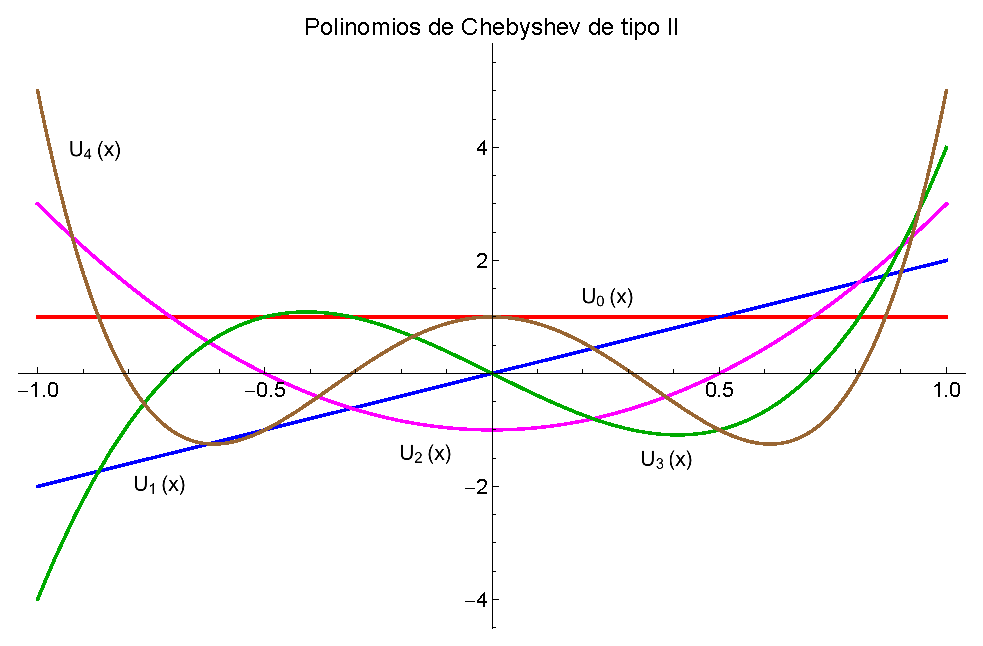
\includegraphics[scale=0.62]{Imagenes/Gram_Schmidt_Chebyshev_2.eps}
\end{figure}
\end{frame}

\section{Problemas Sturm-Liouville}
\frame{\frametitle{Temas a revisar} \tableofcontents[currentsection, hideothersubsections]}
\subsection{Interpretación física}

\begin{frame}
\frametitle{¿De dónde surgen estos problemas?}
Los sistemas Sturm-Liouville surgen típicamente de problemas de \textocolor{cobalt}{vibración} en la mecánica continua.
\\
\bigskip
\pause
En lenguaje físico, describen problemas de frontera correspondientes a ondas estacionarias simplemente armónicas.
\end{frame}
\begin{frame}
\frametitle{Suposiciones clásicas}
Comúnmente suponemos en física que cualquier movimiento ondulatorio se puede resolver en ondas estacionarias simplemente armónicas, cada una de las cuales oscila periódicamente con su frecuencia adecuada.
\end{frame}
\begin{frame}
\frametitle{Apoyo para respaldar las suposiciones}
Aunque los físicos comúnmente asumimos este resultado sobre la base de la evidencia experimental y la intuición, \pause en realidad se puede deducir rigurosamente de la teoría matemática del movimiento ondulatorio como un problema de frontera en las ecuaciones diferenciales.
\end{frame}
\begin{frame}
\frametitle{Tres ejemplos}
Veamos la interpretación física de las eigenfunciones de los sistemas de Sturm Liouville con tres ejemplos clásicos.
\end{frame}

\subsection{Ecuación de onda}

\begin{frame}
\frametitle{La ecuación de onda}
La EDP de una cuerda que vibra es:
\pause
\begin{align*}
\pdv[2]{y}{t} = c^{2} \, \pdv[2]{y}{x} \hspace{1.3cm} c^{2} = \dfrac{T}{\rho}
\end{align*}
\pause
Donde:
\setbeamercolor{item projected}{bg=carnelian,fg=white}
\setbeamertemplate{enumerate items}{%
\usebeamercolor[bg]{item projected}%
\raisebox{1.5pt}{\colorbox{bg}{\color{fg}\footnotesize\insertenumlabel}}%
}
\begin{enumerate}[<+->]
\item $y$ es el desplazamiento lateral desde el punto de equilibrio.
\item $T$ es la tensión (constante)
\item $\rho$ la densidad de la cuerda (constante)
\end{enumerate}
\end{frame}
\begin{frame}
\frametitle{Separando la ecuación de onda}
Las ondas estacionarias simplemente armónicas se definen por la separación de variables:
\begin{align*}
y (x, t) = u (x) \, \cos k(t - t_{0})
\end{align*}
\end{frame}
\begin{frame}
\frametitle{Solución a la ecuación de onda}
Para que la solución $y (x, t)$ satisfaga la ecuación de onda $y_{tt} = c^{2} \, y_{xx}$, \pause \textocolor{bole}{es necesario y suficiente} que:
\begin{align*}
\sderivada{u} + \lambda \, u = 0, \hspace{1.3cm} \lambda = \dfrac{k^{2}}{c^{2}}
\end{align*}
donde $k$ depende de la condición del extremo final.
\end{frame}
\begin{frame}
\frametitle{Condición natural en la cuerda}
Para la cuerda que vibra, \pause \textocolor{byzantine}{es natural físicamente tener extremos fijos}, de modo que:
\pause
\begin{align*}
y (a, t) = y (b, t) = 0
\end{align*}
\pause
Esto hace que:
\begin{align*}
u (a) = u (b) = 0
\end{align*}
\end{frame}
\begin{frame}
\frametitle{Los eigenvalores}
El eigenvalor perteneciente a cada eigenfunción \textocolor{cerise}{es proporcional} a la frecuencia al cuadrado $k^{2}/4 \pi^{2}$.
\\
\bigskip
\pause
Esta relación, combinada con la analogía entre ondas mecánicas y electromagnéticas, ha llevado a los matemáticos a llamar al conjunto de eigenvalores como \textcolor{blue}{el espectro} de un sistema S-L.
\end{frame}

\subsection{Vibraciones en una barra}

\begin{frame}
\frametitle{El caso de una barra elástica}
Otra \textocolor{burgundy}{interpretación física} de los sistemas S-L la proporcionan \textcolor{ao(english)}{las vibraciones longitudinales de una barra elástica} de rigidez local $p (x)$ y densidad $p (x)$.
\end{frame}
\begin{frame}
\frametitle{La ecuación de onda para la barra}
El desplazamiento longitudinal medio $v (x, t)$ de la sección de dicha barra desde su posición de equilibrio $x$ satisface la ecuación de onda:
\pause
\begin{align*}
\rho (x) \, \pdv[2]{v}{t} = \pdv{x} \bigg[ p (x) \, \pdv{v}{x} \bigg]
\end{align*}
\end{frame}
\begin{frame}
\frametitle{Oscilaciones armónicas}
Las oscilaciones armónicas simples (los \textocolor{carmine}{modos normales} de oscilación) están dados por la separación de variables:
\pause
\begin{align*}
v (x, t) = u (x) \, \cos k(t - t_{0})
\end{align*}
\end{frame}
\begin{frame}
\frametitle{Oscilaciones armónicas}
Que son soluciones a la ecuación de S-L:
\pause
\begin{align*}
\dv{x} \bigg[ p (x) \, \dv{u}{x} \bigg] + k^{2} \, \rho (x) \, u = 0
\end{align*}
En este caso especial, $q = 0$ y $\lambda = k^{2}$.
\end{frame}
\begin{frame}
\frametitle{CDF para una barra finita}
Para una barra finita, que se extiende en el intervalo $a \leq x \leq b$, se presentan naturalmente varias condiciones físicas de frontera:
\pause
\setbeamercolor{item projected}{bg=darkblue,fg=white}
\setbeamertemplate{enumerate items}{%
\usebeamercolor[bg]{item projected}%
\raisebox{1.5pt}{\colorbox{bg}{\color{fg}\footnotesize\insertenumlabel}}%
}
\begin{enumerate}[<+->]
\item $u (a) = u (b) = 0$ extremos rígidamente fijos
\item $\pderivada{u} (a) = \pderivada{u} (b) = 0$ extremos libres
\item $\pderivada{u} (a) + \alpha u (a) = \pderivada{u} (b) + \beta u (b) = 0$ extremos sujetos elásticamente
\item $u (a) = u (b) \hspace{0.5cm} \pderivada{u} (a) = \pderivada{u} (b)$ restricciones periódicas
\end{enumerate}
\end{frame}
\begin{frame}
\frametitle{Las condiciones en la solución}
Cada una de estas condiciones de punto final en $u$ \textocolor{darkmagenta}{implica una condición correspondiente} en $v (x, t)$, con $\dv*{x}$ reemplazada por $\pdv*{x}$.
\end{frame}
\begin{frame}
\frametitle{Frecuencias naturales}
Las frecuencias naturales de vibración longitudinal (\textcolor{lava}{tono musical fundamental} y \textcolor{blue}{sobretonos}) de una barra cuyos extremos se mantienen en cada una de las formas descritas son, \pause por lo tanto, las soluciones de los sistemas S-L y las condiciones apropiadas anteriores.
\end{frame}

\subsection{Membrana oscilante}

\begin{frame}
\frametitle{Una membraba oscilando}
La EDP de una membrana oscilando es:
\begin{align*}
w_{tt} = c^{2} \, (w_{xx} + w_{yy}) = c^{2} \, (w_{rr} + r^{-1} \, w_{r} + r^{2} \, w_{\theta \theta})
\end{align*}
donde $r$, $\theta$ indican las coordenadas polares.
\end{frame}
\begin{frame}
\frametitle{Solución al problema}
Se puede encontrar una base de soluciones de onda estacionaria mediante la separación de variables:
\begin{align*}
w (r, \theta, t) = u (r) \, \left\{ \stackrel{\displaystyle \cos}{\sin} \right\} \, n \, \theta \, \cos \kappa (t - t_{0})
\end{align*}
\end{frame}
\begin{frame}
\frametitle{Requisito para la solución}
Para que $w$ satisfaga la ecuación de membrana con $\kappa = c \, k$, \pause es \emph{necesario y suficiente} de que $u$ sea una solución de la ecuación de Bessel.
\\
\bigskip
\pause
La singularidad en $r = 0$ de la ecuación de Bessel está asociada con la singularidad en coordenadas polares en el origen.
\end{frame}
\begin{frame}
\frametitle{Cuando la membrana es un parche}
Si la membrana es un disco circular de radio $a$ (como el parche de un tambor), \pause las condiciones de frontera físicamente naturales son $u (a) = 0$ y $u(0)$ no singular.
\\
\bigskip
\pause
La última condición caracteriza las funciones de Bessel entre otras soluciones de la ecuación de Bessel, hasta un factor de normalización constante.
\end{frame}
\end{document}